\documentclass[12pt,a4paper]{article}
\usepackage{cmap}
\usepackage[slovak]{babel}
\usepackage[utf8]{inputenc}
\usepackage[T1]{fontenc}

\usepackage{amsmath}
\usepackage{amssymb}
\usepackage{lmodern}
\usepackage{indentfirst}
\usepackage{hyperref}
\usepackage{enumitem}
\usepackage{graphicx}
\usepackage{float}
\usepackage{titlesec}

\setcounter{secnumdepth}{4}

\titleformat{\paragraph}
{\normalfont\normalsize\bfseries}{\theparagraph}{1em}{}
\titlespacing*{\paragraph}
{0pt}{3.25ex plus 1ex minus .2ex}{1.5ex plus .2ex}

\begin{document}
	
\begin{titlepage}
	\centering
	\vspace{1cm}
	{\scshape\LARGE UnixMotion} \par
	\vspace{1cm}
	{\huge\bfseries Kvantovo-chemické výpočty} \par
	\vspace{2cm}
	{\Large\itshape Jaroslav Ištok \par}
	{\Large\itshape Katarína Fabianová \par}
	{\Large\itshape Dušan Suja \par}
	{\Large\itshape Jerguš Adamec \par}
	\vfill
	\begin{figure}[H]
		\centering
		
\includegraphics[width=0.4\textwidth]{fmfi}
	\end{figure}
	\vspace{2cm}
	{\large FMFI AIN}
\end{titlepage}

\pagebreak

\tableofcontents
\vspace{2cm}
\listoffigures

\pagebreak

\section{Špecifikácia požiadaviek}

\subsection{Úvod}

\subsubsection{Účel}
Špecifikácia obsahuje všetky požiadavky, ktoré bude aplikácia implementovať. Je určená všetkým, ktorí sa budú podielať na vývoji, zahŕňajúc zadávateľa, ktorý kontroluje, či spísané požiadavky spĺňajú všetky potreby, ktoré na systém má, manažérov vývojového tímu, ktorí ju využívajú pri plánovaní a riadení procesu vývoja, dizajnérov, ktorí podľa nej vytvárajú návrh aplikácie, vývojárov, ktorí postupujú podľa návrhu, ktorý sa na ňu odkazuje a pomáha im pochopiť aplikáciu, ktorú vyvíjajú, tvorcov testov, ktorí podľa nej vytvárajú validačné testy, správcov výslednej aplikácie, ktorí podľa nej vykonávajú údržbu systému po jeho dodaní. Výsledná špecifikácia je pre všetkých zúčastnených čitateľná a zrozumiteľná.

\subsubsection{Rozsah projektu}
Projekt sa radí medzi stredne veľké projekty. Jeho vývoj bude prebiehať v časovom horizonte približne pol roka, pričom jeho samotná implementácia bude prebiehať v rozsahu jedneho mesiaca. Obsah aplikácie bude pozostávať z častí ako sú crawler, lexer, parser, ORM a jednoduchého, no súčasne intuitívneho grafického užívateľského rozhrania.

\subsubsection{Definície, akronymi a skratky}
\begin{itemize}
	\item Crawler - nástroj, ktorý prelieza adresáre na serveroch a hľadá súbory
	\item Lexer - nástroj, ktorý analyzuje štruktúru súboru (dokumentu)
	\item Parser - nástroj na spracovanie údajov zo súborov
	\item ORM - nástroj na prácu s databázou z programovacieho jazyka
\end{itemize}

\subsubsection{Odkazy}
\begin{itemize}
	\item Priklad zobrazenia spracovaných dát: \url{http://neon.dpp.fmph.uniba.sk/qch_calcs/index.php}
\end{itemize}

\subsubsection{Prehľad zostávajúcej časti dokumentu}
V nasledujúcich kapitolách nájdete rozširujúce informácie o projekte. Všeobecný popis projektu, perspektívu projektu, podrobný popis funkcionality, účel projektu, charakteristiku cieľových používateľov projektu a ďaľšie.

\subsection{Všeobecný popis}
Výsledná aplikácia bude spravovať a prehľadávať databázu, obsahujúcu výsledky kvantovo-chemických výpočtov a bude pravidelne aktualizovaná automaticky alebo manuálne na vyžiadanie samotného používateľa. Aplikácia bude prístupná len vybraným používateľom, ktorým bude pridelené ich vlastné prihlasovacie meno a heslo. Každému z používateľov bude zároveň prístupný celý obsah databázy, teda obsah spravovaný každým z jednotlivých používateľov. Samotná aplikácia sa bude vyznačovať vysokou prenosnosťou vzhľadom na nulovú veľkosť a z toho vyplývajúce nulové požiadavky na dostupnú kapacitu pamäte, s dôrazom na vysokú dostupnosť vyplývajúcu z prístupu cez príslušnú webstránku.

\subsubsection{Perspektívny pohľad na projekt}
Projekt bude mať otvorený zdrojový kód. Bude bežať na linuxovom serveri a bude poskytovať webové rozhranie.

\subsubsection{Funkcionalita výslednej aplikácie}
\begin{itemize}
	\item Aplikácia vyhľadá súbory s výsledkami výpočtov z meracích prístrojov, ktoré sú uložené na konkrétnych serveroch. Dáta zo súborov najskôr analyzuje, potom spracuje a uloží ich do databázy.
	\item Aplikácia v pravidelných časových intervaloch, alebo na vyžiadanie používateľa, bude rozširovať databázu o dáta z novopridaných súborov.
	\item Aplikácia poskytne používateľovi jednoduché a intuitívne webové rozhranie, v ktorom bude možné vykonávať požadované operácie nad dátami z databázy, ako je napríklad pokročilé vyhľadávanie na základe rôznych kritérii. Webové rozhranie bude vedieť poskytnúť informácie o určitej molekule, či bola niekedy analyzovaná, akými metódami bola analyzovaná a podobne.
	\item Na prácu s aplikáciou postačí pripojenie na internet a webový prehliadač.
	\item Aplikácia bude chránená heslom a každý používateľ bude mať svoje prihlasovacie údaje, ktoré bude možné zmeniť.
\end{itemize}

\subsubsection{Charakteristika používateľov}
Aplikácia je určená pre chemikov a fyzikov, ktorí pracujú s veľkým množstvom dát z meracích prístrojov a potrebujú v nich mať poriadok. Zákazníci sú profesionálni chemici a fyzici, ktorí potrebujú nástroj, ktorý by im zjednodušil prácu s dátami analyzovaných molekúl.

\subsubsection{Všeobecné obmedzenia}
\begin{itemize}
	\item Aplikácia je robená na mieru, takže nemôže si hocikto vytvoriť účet a používať ju.
	\item Na využívanie aplikácie je potrebné mať prístup k internetu a webový prehliadač.
	\item Webové rozhranie zobrazuje len molekuly, ktoré sú uložené v databáze.
	\item Ak je výpočet pre nejakú molekulu neúplný alebo chybný, potom danú molekulu nebude možné zobraziť. Objaví sa iba upozornenie, že dáta z výpočtu nie sú validné.
	\item Ak hľadaná molekula neexistuje v databáze, používateľ má možnosť nahrať súbor s výpočtom pre danú molekulu a v nasledujúcom vyhľadávaní, údaje o molekule budú zobrazené.
\end{itemize}

\subsubsection{Predpoklady a závislosti}
Grafické užívateľské prostredie bude po otvorení webstránky s aplikáciou v úvode pozostávať z prihlasovacieho formuláru tvoreného textovými poľami, určenými pre zadanie používateľského mena a používateľského hesla, slúžiacimi na identifikáciu jednotlivých vybraných používateľov. \par
Po prihlásení bude používateľovi zobrazený aktuálny výpis údajov obsiahnutých v databáze, ako aj prvky ovládačov, slúžiacich na prácu s vybranými dátami, podľa bližšie špecifikovaných požiadaviek zadávateľa.

\subsection{Zoznam špecifických požiadaviek na systém}
\begin{enumerate}[label={[\arabic*]}]
	\item{\bf Vyhľadávanie súborov na serveroch} \par 
	Aplikácie bude vyhľadávať súbory na serveroch, ktoré obsahujú výsledky výpočtov z meracích zariadení. Tieto súbory bude ďalej spracovávať. Konkrétne miesta vyhľaávania budú špecifikované v konfiguračných súboroch.
	\item{\bf Analýza nájdených súborov} \par
	Aplikácia bude analyzovať nájdené súbory, resp. bude zisťovať či majú validnú štruktúru, vhodnú k ďalšiemu spracovaniu.
	\item{\bf Spracovanie údajov z nájdených súborov} \par
	Aplikácia bude vedieť spracovať dáta z nájdených súborov do vhodného formátu, aby ich bolo možné ľahko uložiť do databázy. 
	\item{\bf Uloženie údajov do databázy} \par
	Aplikácia bude vedieť uložiť spracované dáta prehľadne do databázy. S dátami v databáze sa bude dať ďalej pracovať.
	\item{\bf Aktualizovanie databázy o novopridané súbory} \par
	Aplikácia bude v pravidelných časových intervaloch, alebo na vyžiadanie používateľa,  zisťovať prítomnosť novopridaných súborov, ktorých údaje ešte nie sú uložené v databáze a aktualizovať databázu o nové údaje.
	\item{\bf  Webové používateľské rozhranie} \par
	Aplikácia bude ovládaná pomocou jednoduchého webového používateľského rozhrania.
	\item{\bf Možnosť vykonávania operácii nad dátami v databáze} \par
	Aplikácia bude poskytovať nástroje na prácu s údajmi uloženými v databáze. Bude medzi nimi vedieť vyhľadávať podľa rôznych kritérii, zisťovať informácie o tom, či bola konkrétna molekula analyzovaná, resp. či sa nachádza v databáze. Keď nájde požadovanú molekulu, vypíše, akými metódami bola analyzovaná, koľko krát bola analyzovaná a podobne.
	\item{\bf Zabezpečenie aplikácie} \par
	Na prístup do aplikácie bude nutné prihlásenie svojim používateľkým menom a heslom.
\end{enumerate}

\section{Návrh}

\subsection{Diagramy}

\subsubsection{Entitno-relačný diagram}
\begin{figure}[H]
	\caption{Entitno-relačný diagram}
	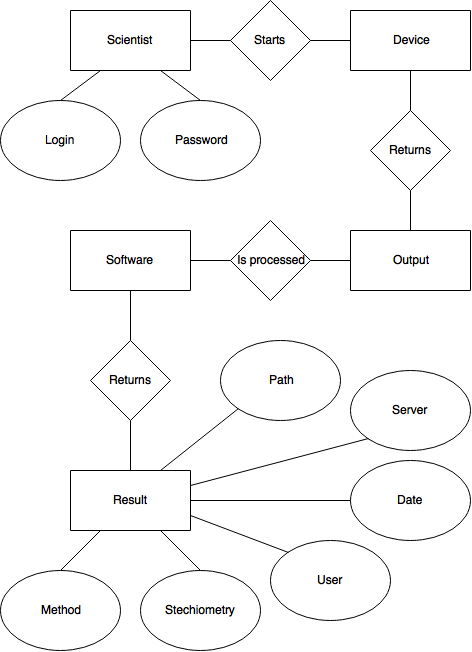
\includegraphics[width=\textwidth]{er_diagram}
	\label{fig:er_diagram}
\end{figure}
\ref{fig:er_diagram}
Entitno-relačný diagram znázorňuje vzťahy (relácie) medzi entitami. Diagram je použitý na modelovanie priestoru domény, pre ktorú sa informačný systém vyvíja (ústav experimentálnej fyziky). Entity sú zakreslené do obdĺžnikov. Vzťahy (relácie) medzi entitami sú v kosoštvorcoch, sú prepojené so všetkými entitami, ktoré do daného vzťahu vstupujú a sú pomenované. Entity majú svoje atribúty, ktoré sú do diagramu zakreslené ako ovály spojené so svojou entitou úsečkou.

\subsubsection{Use-case diagram}
\begin{figure}[H]
	\caption{Use-case diagram}
	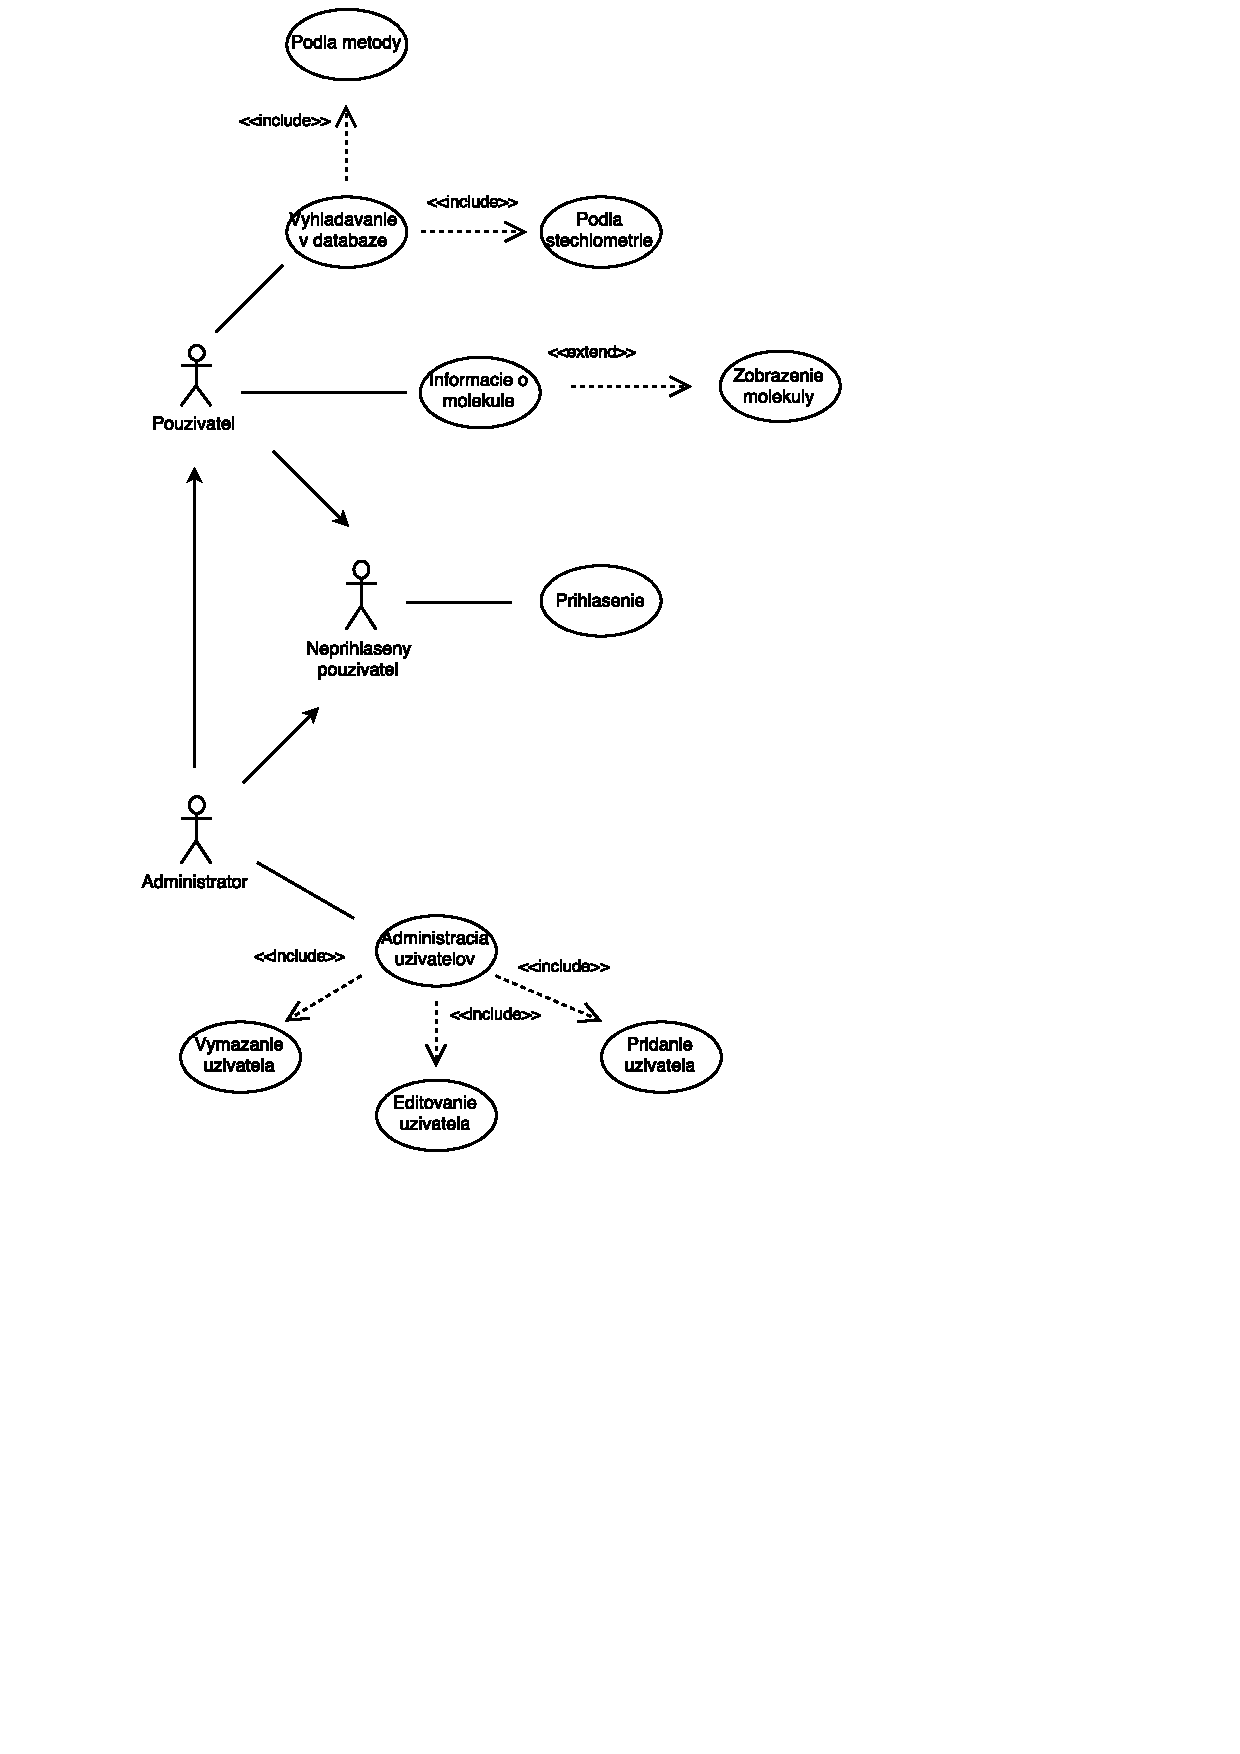
\includegraphics[width=\textwidth]{use-case}
	\label{fig:use_case}
\end{figure}
\ref{fig:use_case}
Use-case diagram popisuje interakciu používateľov (aktorov) s aplikáciou. Neprihlásený používateľ sa môže prihlásiť. Prihlásený používateľ môže vyhľadávať v databáze výsledkov meraní podľa rôznych kritérii, či zobraziť výpis podrobných informácii o danej molekule a tiež zobraziť jej náhľad.

\subsubsection{Stavový diagram}
\begin{figure}[H]
	\caption{Stavový diagram}
	\includegraphics[width=\textwidth]{state}
	\label{fig:state}
\end{figure}
\ref{fig:state}
Stavový diagram popisuje proces spracovania súboru aplikáciou. Spracovanie sa začína otvorením súboru a jeho následnou prvotnou analýzou (validáciou). V prípade, že súbor nie je validný, tak sa nepokračuje ďalej v jeho spracovaní. V prípade, že súbor je validný sa zistí, či má súbor windowsový alebo linuxový formát. Tieto dva formáty sa líšia vnútornou štruktúrou a teda aj spôsobom spracovania. Zo súboru sa následne vyparsujú potrebné dáta a spracovanie súboru skončí jeho zatvorením. 

\subsubsection{Sekvenčný diagram - spracovanie súboru}
\begin{figure}[H]
	\caption{Sekvenčný diagram - spracovanie súboru}
	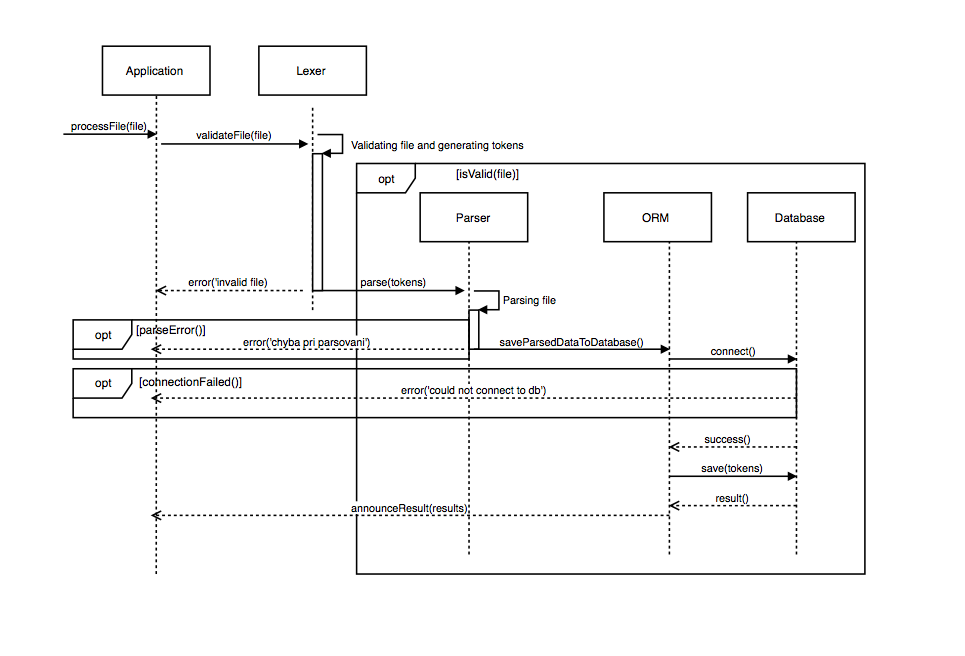
\includegraphics[width=\textwidth]{sequence_file}
	\label{fig:seq}
\end{figure}
\ref{fig:seq}
Diagram popisuje komunikáciu komponentov našej aplikácie počas spracovania súboru. Na začiatku aplikácia pošle lexeru požiadavku na validáciu súboru. Lexer súbor zvaliduje a rozparsuje na tokeny, v prípade chyby, pošle hlavnému programu správu s chybou. Tokeny pošle parseru, ktorý ich rozparsuje. Dáta z parseru sa pošlú ORM-ku, ktoré sa pripojí k databáze a uloží do nej naparsované dáta. Na konci pošle správu o úspechu, resp. neúspechu celej operácie do hlavného programu, ktorý ju spracuje.

\subsubsection{Sekvenčný diagram -  pripojenie k databáze}
\begin{figure}[H]
	\caption{Sekvenčný diagram - pripojenie k databáze}
	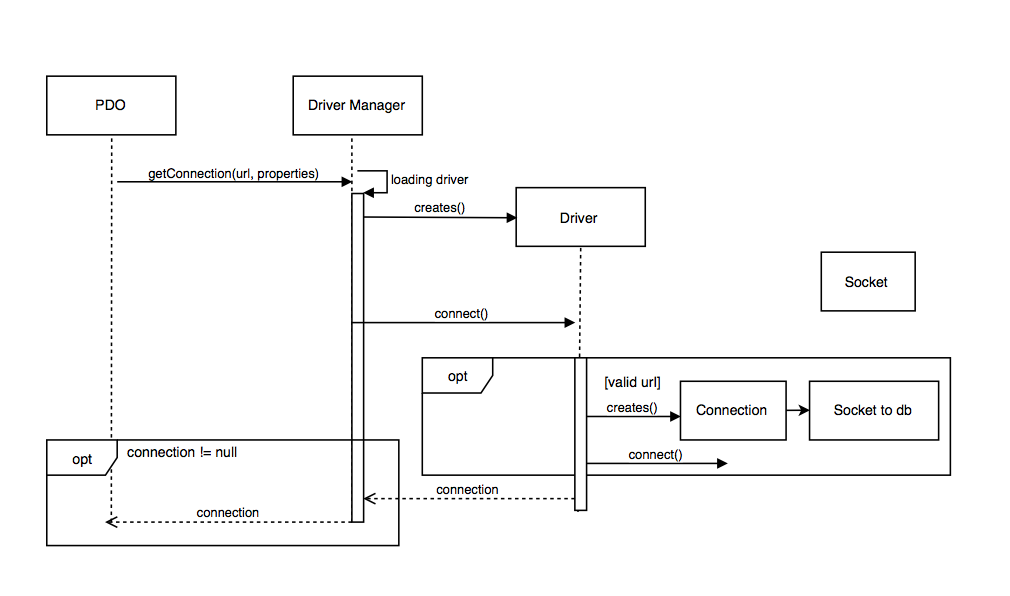
\includegraphics[width=\textwidth]{db}
	\label{fig:db}
\end{figure}
\ref{fig:db}
Diagram popisuje proces pripojenia k databáze. Knižnica PDO pošle požiadavku na získanie spojenia k databáze driver manageru. Ten načíta drivre, vyberie správny a vytvorí jeho inštanciu. Driver sa následne pokúsi vytvoriť spojenie k databáze, tým, že sa pokúsi pripojiť na socket. V prípade neúspechu sa pošle správa do PDO o neúspechu. V prípade úspešného pripojenia na socket sa vráti spojenie k databáze do PDO.

\subsubsection{Dátový model}
\begin{figure}[H]
	\caption{Dátový model}
	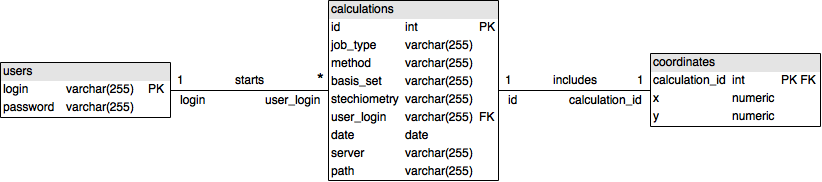
\includegraphics[width=\textwidth]{datovy_model}
	\label{fig:datovy_model}
\end{figure}
\ref{fig:datovy_model}
Dátový model popisuje štruktúru databázy.
\begin{itemize}
	\item{\bf Users} \par
	Tabuľka users obsahuje zoznam používateľov. Používatelia majú priradené id, plniace funkciu primárneho kľúča (id), meno, pod ktorým sa prihlasujú (login) a heslo, s ktorým sa prihlasujú (password).
	\item{\bf Calculation results} \par
	Tabuľka calculation results obsahuje zoznam výsledkov výpočtov. Výsledky výpočtov majú priradené id, plniace funkciu primárneho kľúča (id), spôsob testovania vzorky (job type), metódu testovania vzorky (method), iniciálnu konfiguráciu (basis set), zjednodušený chemický vzorec testovanej vzorky (stechiometry), používateľa, spúšťajúceho testovanie vzorky (user), dátum testovania vzorky (date), meno servera, ukladajúceho daný výsledok výpočtu (server) a cestu k súboru daného výsledku výpočtu (path).
	\item{\bf History} \par
	Tabuľka history obsahuje zoznam spracovaných súborov. Spracované súbory majú priradené id, plniace funkciu primárneho kľúča (id) a cestu, ktorá popisuje ich umiestnenie (path).
	\item{\bf Logs} \par
	Tabuľka logs obsahuje zoznam chybových správ. Chybové správy majú priradené id, plniace funkciu primárneho kľúča (id) a text, ktorý je ich obsahom (text).
\end{itemize}

\subsubsection{Komponentný diagram}
Komponentný diagram popisuje dekompozíciu projektu na moduly.
\begin{itemize}
	\item{\bf Autorizácia} \par
	Pomocou komponentu autorizácia sa budúci používateľ správnym vyplnením prihlasovacieho formulára prihlási do systému. Údaje z formulára sa porovnajú s údajmi v databáze. Pri zhode sa používateľ prihlási do systému, kde má k dispozícií rôzne jeho funkcionality.
	\item{\bf Crawler} \par
	Komponent Crawler bude vyhľadávať súbory s výsledkami výpočtov z meracích prístrojov, ktoré sú uložené na konkrétnych serveroch.
	\item{\bf Spracovanie súboru} \par
	Komponent spracovanie súboru zanalyzuje (zistí či súbory majú valídnu štruktúru) a následne spracuje vyhľadané súbory do vhodného formátu.
	\item{\bf Databáza} \par
	Komponent databáza má na starosti pripojenie a prácu s databázou.
\end{itemize}

\subsubsection{Domain-level class diagram}


\subsubsection{Data-flow diagram}


\subsubsection{Triedny diagram}
\begin{figure}[H]
	\caption{Triedny diagram}
	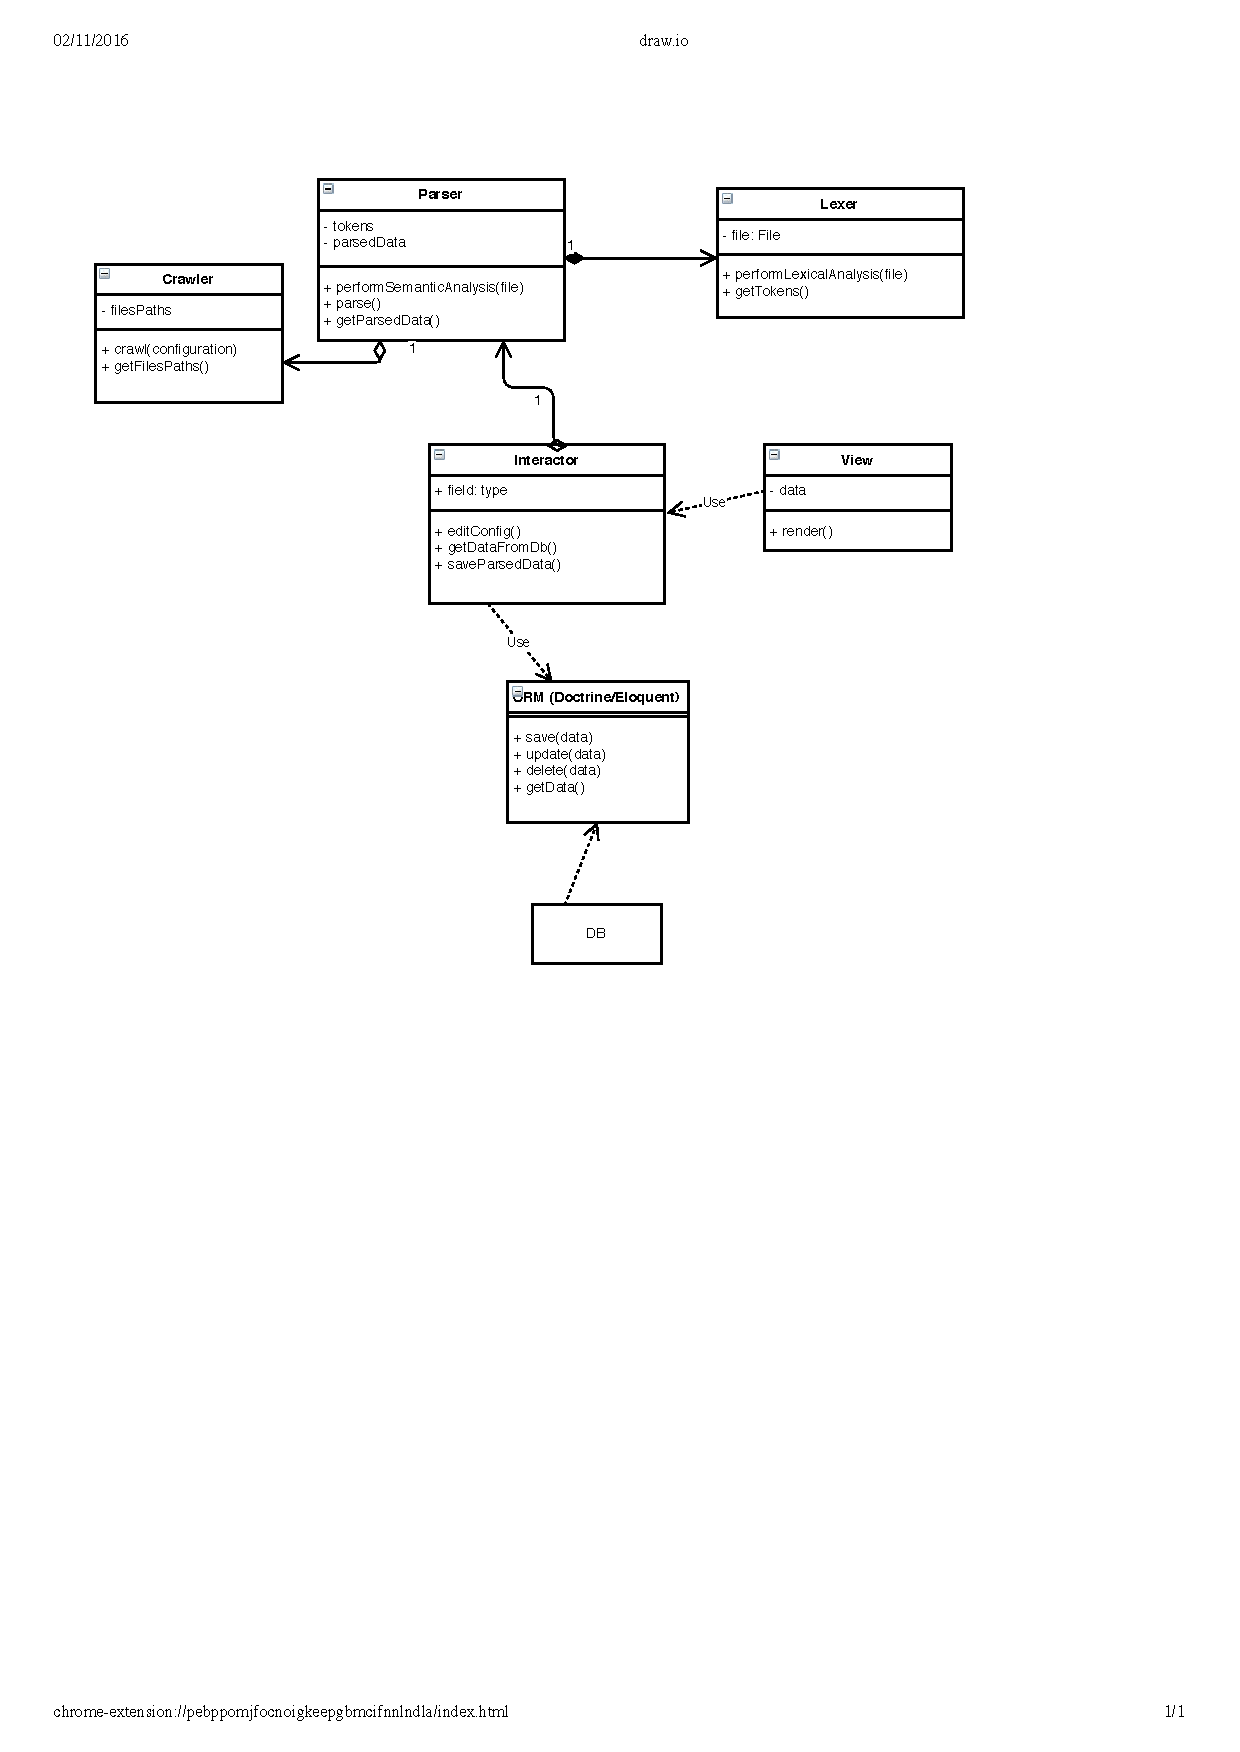
\includegraphics[width=\textwidth]{class_diagram}
	\label{fig:class_diagram}
\end{figure}
\ref{fig:class_diagram}
Triedny diagram modeluje jednotlivé triedy a vzťahy medzi nimi. Každá entita triedneho diagramu popisuje triedu, jej základné atribúty a metódy. Medzi triedami sú šípky, ktoré reprezenutujú jednotlivé vzťahy. Parser bude používať Crawler na vyhľadanie súborov a rovanko bude používať aj Lexer, pomocou, ktorého spraví lexikálnu analýzu súboru. Interactor bude akési spojítko jednotlivých hlavných častí aplikácie. View-u bude poskytovať dáta na zobrazenie a Parseru poskytne prístup k databáze.

\subsection{Používateľské rozhranie}
Používateľké rozhranie aplikácie je navrhnuté jednoducho podľa požiadaviek zadávateľa projektu.
\begin{figure}[H]
	\caption{Obrazovka s prihlásením}
	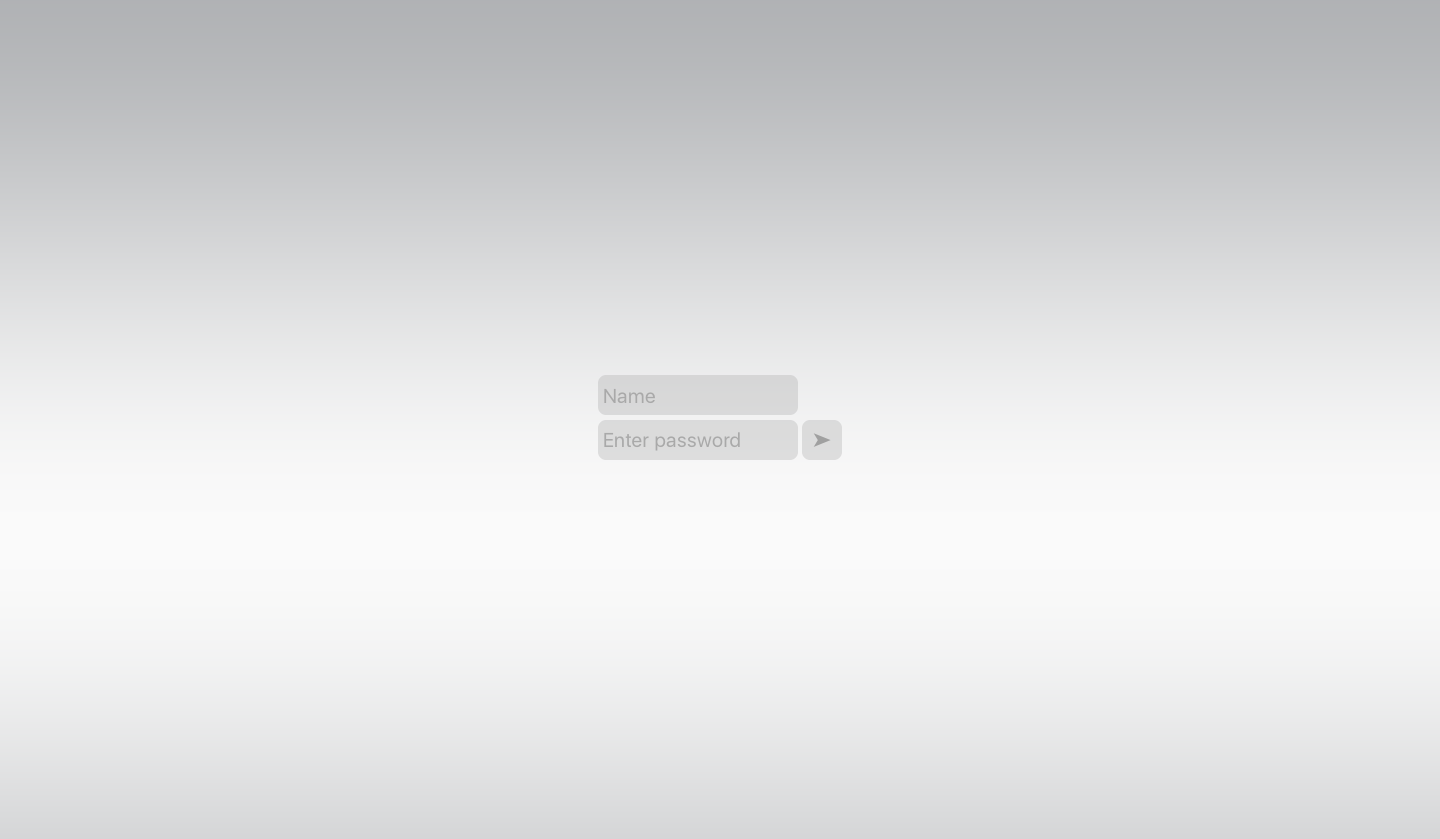
\includegraphics[width=\textwidth]{login}
	\label{fig:ui1}
\end{figure}
\ref{fig:ui1}
Úvodná obrazovka s prihlásením pozostáva z prihlasovacieho formuláru tvoreného textovými poľami, určenými pre zadanie používateľského mena a používateľského hesla, slúžiacimi na identifikáciu jednotlivých vybraných používateľov.
\begin{figure}[H]
	\caption{Obrazovka s tabuľkou výpočtov}
	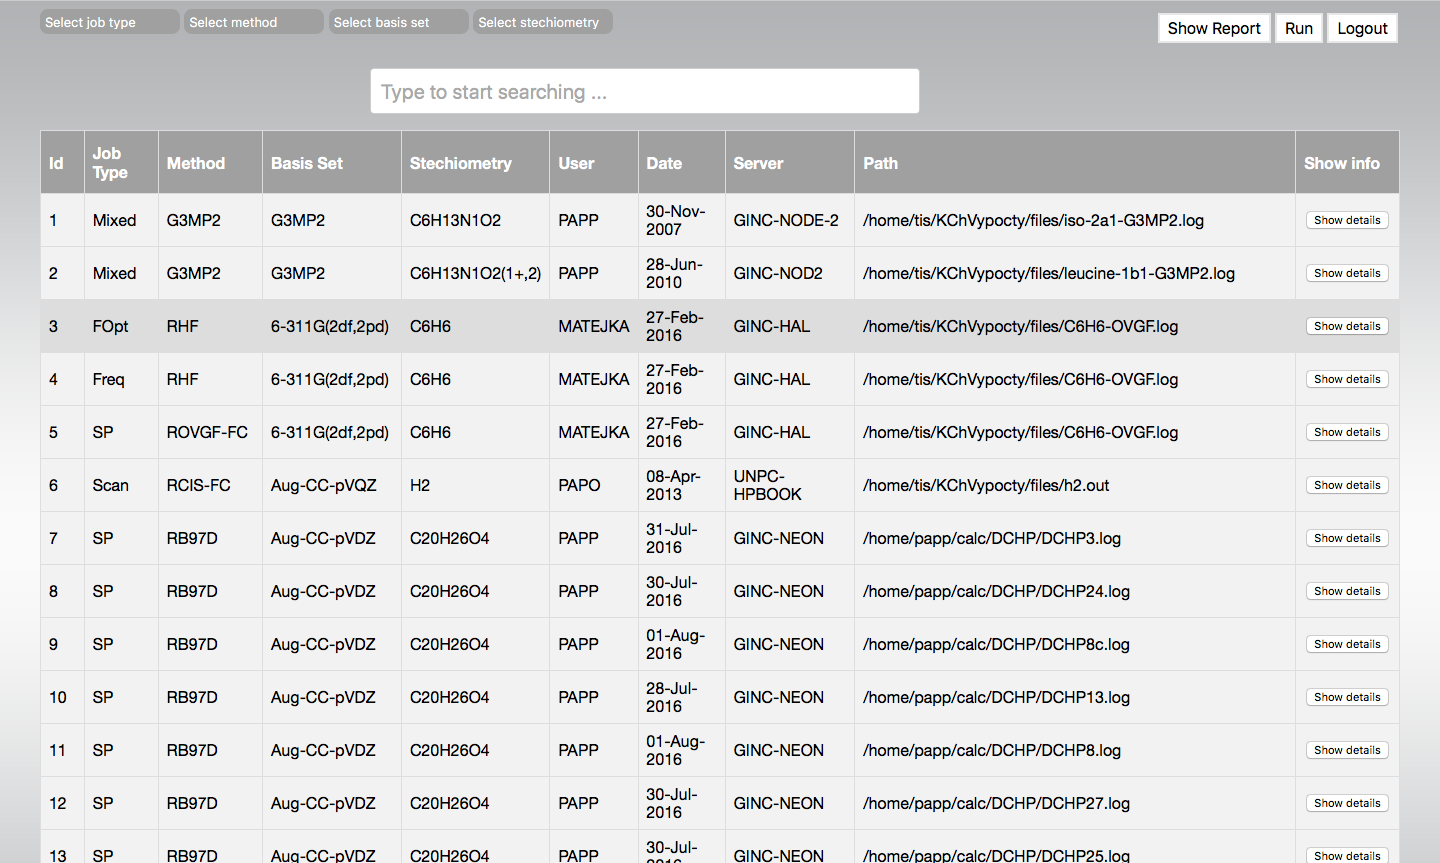
\includegraphics[width=\textwidth]{table}
	\label{fig:ui2}
\end{figure}
\ref{fig:ui2}
Obrazovka s tabuľkou výpočtov po prihlásení používateľovi zobrazuje formou tabuľky aktuálny výpis údajov výpočtov obsiahnutých v databáze, prvky ovládačov, slúžiacich na vyhľadávanie týchto údajov formou textového poľa, ako aj ovládačov, slúžiacich na prácu s vybranými dátami formou tlačidiel.
\begin{figure}[H]
	\caption{Obrazovka s výpočtom}
	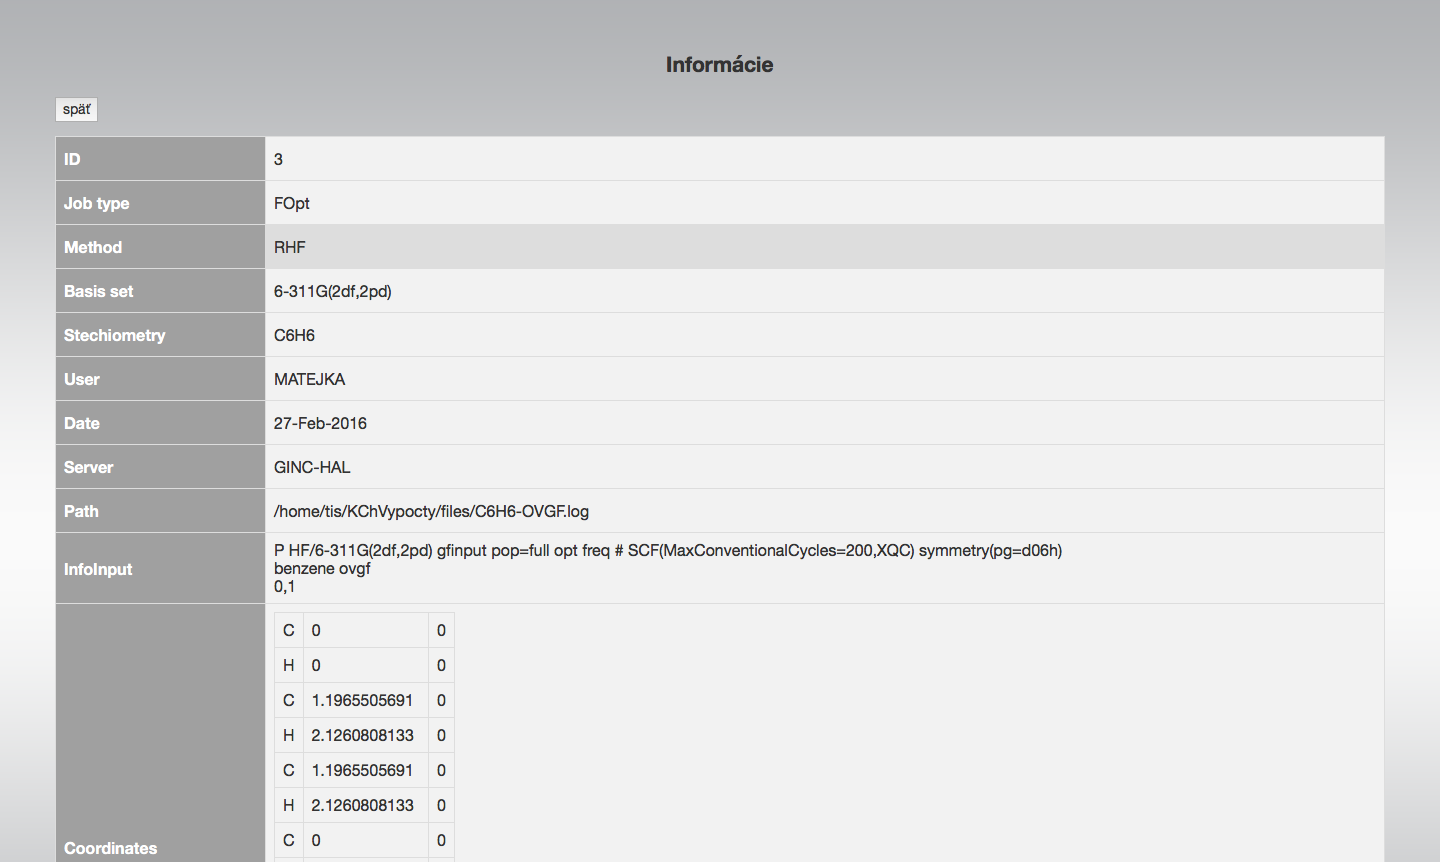
\includegraphics[width=\textwidth]{item}
	\label{fig:ui3}
\end{figure}
\ref{fig:ui3}
Obrazovka s výpočtom po aktivovaní prvku ovládača vo forme tlačidla, určeného pre zobrazenie podrobností konkrétneho výpočtu, používateľovi zobrazuje formou tabuľky aktuálny výpis detailných informácií o danom výpočte obsiahnutých v databáze.

\subsection{Analýza technológií}

\subsubsection{Výber programovacieho jazyka}
Pri výbere programovacieho jazyka sme sa rozhodovali medzi Python-om a PHP. Vybrali sme si PHP, pretože je pre tento projekt najvhodnejší. Medzi výhody, ktoré nám ponúka pri vývoji patria napríklad:
\begin{itemize}
	\item Patrí medzi najpoužívanejšie jazyky vo webových aplikáciach.
	\item Je predinštalovaný na serveri, na ktorom bude bežať aj naša aplikácia.
	\item Plne podporuje objektovo orientované programovanie.
	\item V PHP je na výber veľa kvalitných frameworkov na prácu s databázou.
	\item Vieme s ním efektívne pracovať.
\end{itemize}
Python je náročnejšie nakonfigurovať na webovom serveri, kde pravdepodobne nebudeme mať možnosť inštalácie nového softwéru a oproti PHP ponúka len málo výhod pre náš projekt. Žiadnu podstatnú výhodu nám Python neponúka.

\subsubsection{Výber databázového systému}
Pri výbere databázového systému sme sa rozhodovali medzi Mysql a PostgreSql. PostgreSql ponúka veľa pokročilých funkcii, ako napríklad rekurzívne dopyty, pohľady. Naša aplikácia bude obsahovať jednoduchú databázu s malým počtom tabuliek a tieto pokročilé funkcie nevyužijeme. Preto sme si vybrali mysql databázu, ktorá je predinštalovaná na serveri a jej databázové enginy sú optimalizované pre webové aplikcie.

\subsubsection{Výber ostatných technológií}
\begin{itemize}
	\item{\bf HTML} \par
	Hypertextový značkový jazyk (HyperText Markup Language; HTML) je značkový jazyk určený na vytváranie webových stránok a iných informácií zobraziteľných vo webovom prehliadači. HTML kladie dôraz skôr na prezentáciu informácií (odseky, fonty, váha písma, tabuľky atď.) ako na sémantiku (význam slov) a umožňuje vytvárať dokumenty obsahujúce text, hypertextové odkazy, multimediálny a iný obsah, formuláre, skripty a metainformácie prehliadateľné v tzv. webovom prehliadači. Jazyk HTML je textový, teda umožňuje čítanie a upravovanie priamo v textovom editore. V projekte bude použitý pri tvorbe webových dokumentov z hľadiska ich obsahu, štruktúry.
	\item{\bf CSS} \par
	Kaskádové štýly (Cascading Style Sheets; CSS) je všeobecné rozšírenie HTML. CSS je jednoduchý mechanizmus na vizuálne formátovanie internetových dokumentov. Pomocou kaskádových štýlov sa vytvárajú štruktúrované dokumenty, teda oddeľuje sa obsah dokumentu (HTML) od jeho vzhľadu (CSS). Získa sa tým prehľadný a jednoduchý kód. CSS je možné presunúť do externých súborov, zmenší sa tým dátová veľkosť a dá sa jedným súborom zmeniť celý štýl stránky, pričom sa nezaručuje rovnaké vykresľovanie vo všetkých prehliadačoch, vzhľadom k rôznym interpretáciam CSS rôznymi prehliadačmi. V projekte budú použité pri tvorbe webových dokumentov z hľadiska ich výzoru.
	\item{\bf JavaScript} \par
	JavaScript je skriptovací programovací jazyk využívaný najmä na vytváranie dynamického obsahu webových stránok. V projekte bude použitý pri tvorbe webových dokumentov z hľadiska ich dynamického obsahu a reagovania na vstup používateľa.
	\item{\bf AJAX} \par
	AJAX (Asynchronous JavaScript + XML) je súhrnné označenie pre technológie vývoja interaktívnych webových aplikácií, ktoré umožňujú meniť obsah stránok bez potreby ich kompletného znovunačítania zo servera. V porovnaní s klasickými webovými aplikáciami môžu AJAX-ové aplikácie pri vhodnom návrhu poskytovať používateľsky komfortnejšíe prostredie, vyžadujú však použitie moderných webových prehliadačov. AJAX nie je samostatný programovací jazyk ani technológia sama o sebe. Je to kombinácia HTML a CSS pre značkovanie a štýlovanie informácií pri zobrazení, DOM spojeného s JavaScriptom pre dynamické zobrazenie a interakciu s prezentovanou informáciou, metódy pre výmenu dát medzi prehliadačom a serverom, bez nutnosti obnovovať zobrazovanú stránku a formátu pre dáta poslané prehliadaču, ktoré môžu byť dynamicky vytvorené skriptom na strane serveru (bežné formáty zahŕňajú XML, predformátované HTML, plain text a JavaScript Object Notation, JSON). V projekte budú použité pri zmene obsahu webových dokumentov bez potreby ich kompletného znovunačítania zo servera.
\end{itemize}

\subsection{Testovacie scenáre}

\subsubsection{Existencia súboru}
Otestovať existenciu súboru a jeho korektné otvorenie. Ak funkcia dostane cestu korektného súboru, so súborom sa dá ďalej pokračovať. V opačnom prípade funkcia súbor zahodí a nepokračuje sa v ďalšom spracovávaní.

\subsubsection{Crawler}
Otestovať funkcionalitu Crawlera. Používateľ pridá nové súbory v používateľskom rozhraní. Crawler má nájsť novopridané súbory a aktualizovať databázu. 

\subsubsection{Validnosť súboru}
Otestovať validnosť súboru. Ak funkcia dostane validný súbor (je v požadovanom formáte), pokračuje sa ďalej v procese. V opačnom prípade, ak funkcia dostane nevalidný vstup (súbor je v zlom formáte), ďalej sa nepokračuje a funkcia súbor zahodí.

\subsubsection{Rozlišovanie linuxových a windowsových súborov}
Otestovať rozlišovanie medzi linuxovým a windowsovým súborom (rozdiel je v type súboru a v pár znakoch). Funkcia rozlíši, či dostala na vstup linuxový alebo windowsový súbor a následne sa súbor parsuje podľa linuxového alebo windowsového formátu.  

\subsubsection{Databáza}
Otestovať pridávanie nových prvkov do databázy. Pridá sa nový korektný súbor a následne treba zistiť, či sa pridal aj do databázy. Pridá sa nový nekorektný súbor a následne treba skontrolovať, či sa údaje zo súboru nepridali do databázy.

\end{document}